% !TeX root = ../ShajiS_RnDDefense.tex

\documentclass[aspectratio=169]{beamer}

\usepackage[utf8]{inputenc}
\usepackage{amsmath}
\usepackage{amsfonts}
\usepackage{amssymb}
\usepackage{graphicx}
\usepackage{ragged2e}  % `\justifying` text
\usepackage{booktabs}  % Tables
\usepackage{tabularx}
\usepackage{tikz}      % Diagrams
\usetikzlibrary{calc, shapes, backgrounds}
\usepackage{amsmath}
\usepackage{amssymb}
\usepackage{dsfont}
\usepackage{url}       % `\url
\usepackage{listings}  % Code listings
\usepackage[T1]{fontenc}
\usepackage[backend=biber, style=ieee, citestyle=numeric-comp, isbn=false, url=false, doi=false, giveninits=true, uniquename=init]{biblatex}
\usepackage{hyperref}
\usepackage{caption}
\usepackage{theme/beamerthemehbrs}
\addbibresource{rnd.bib} % Your bibliography file
\newcommand\blfootnote[1]{%
  \begingroup
  \renewcommand\thefootnote{}\footnote{#1}%
  \addtocounter{footnote}{-1}%
  \endgroup
}
\newcommand\customcolumnwidth{0.4625\textwidth}


% For presentation mode with notes on second screen:
\setbeameroption{show notes on second screen=right}
% For final PDF without notes, comment above line and uncomment below:
% \setbeameroption{hide notes}

\author[Shinas Shaji]{Shinas Shaji}
\title{Evaluation of Few-Shot Transfer of Vision-Language Foundation Models to Learn Lightweight Models for Robotic Vision Tasks}
\subtitle{R\&D Project Defense}
\institute[HBRS]{Hochschule Bonn-Rhein-Sieg}
\date{March 13, 2025}
\subject{R\&D Project Defense}

% leave the value of this argument empty if the advisors
% should not be included on the title slide
\def\advisors{Prof. Dr. Sebastian Houben (Hochschule Bonn-Rhein-Sieg, Fraunhofer IAIS) \\
Santosh Thoduka M.Sc. (Fraunhofer IAIS)}

\thirdpartylogo{theme/images/iais.pdf}

\begin{document}
{
\begin{frame}
\titlepage
\end{frame}
}

\section{Introduction}
\subsection{Background}
\begin{frame}{Introduction}
\framesubtitle{Vision-Language Models (VLMs)}
  \begin{itemize}
    \item Neural networks that process both \emph{images} and \emph{text}
    \item Like Large Language Models (LLMs):
    \begin{itemize}
      \item Learn \emph{general visual-textual understanding} from pre-training~\footfullciteieee{Radford2021}
      \item Then aligned to human preferences and \emph{instruction-following}
    \end{itemize}
    \item Shown to be able to \emph{adapt} to new tasks without extensive task-specific training~\footfullciteieee{Liu2023}, hence quite \emph{generalizable}
    \blfootnote{\vspace{0.05em}}
  \end{itemize}
\end{frame}
\note{
- I know that most of you are already familiar with multi-modal models, being in a room of researchers in multimodal foundation models, but perhaps there are people in the audience who are not familiar with the field. So we start with a brief introduction to some concepts we will be needing today \\ 
- VLMs combine computer vision and natural language processing capabilities in a single neural network \\
- Pre-training occurs on web-scale image-text datasets (e.g., CLIP was trained on 400M image-text pairs). In this way, models learn to understand the relationship between images and text and also predict one from the other \\
- Unlike traditional CV models trained for specific tasks, VLMs learn broader understanding that transfers to many tasks \\
- Similar to how ChatGPT can answer questions on many topics, VLMs can handle multiple visual tasks \\
}


\begin{frame}{Introduction}
\framesubtitle{Few-Shot Transfer}
  \vspace{-1em}
  \begin{itemize}
    \item Teaching a \emph{generalizable model} new tasks by showing it a few \emph{examples}
    \item Model `learns' to recognize patterns from these examples
    \item Can then apply this `learning' to new, unseen instances
  \end{itemize}
  \vspace{-0.2em}
  \begin{columns}[onlytextwidth]
    \column{.5\textwidth}
    % \centering 
    \small{\emph{Prompt}: A [DOG] has droopy ears and is often fluffy. This is a [DOG]:}
    \begin{figure}
      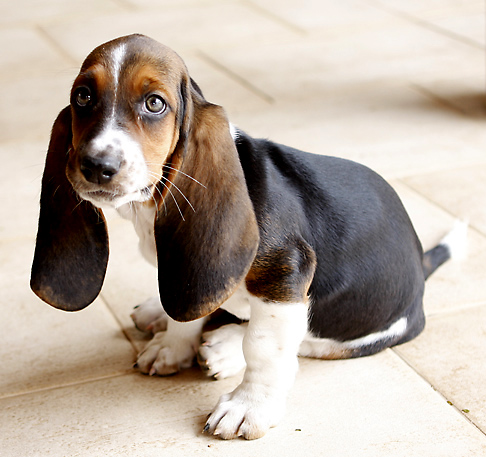
\includegraphics[width=20mm]{./figures/basset-hound.jpeg}
      \caption{\centering This is a [DOG]. \\ \tiny{Image from Wikipedia, \href{https://commons.wikimedia.org/w/index.php?curid=32270218}{Link}}}
    \end{figure}
    \column{.5\textwidth} 
    \begin{figure}
      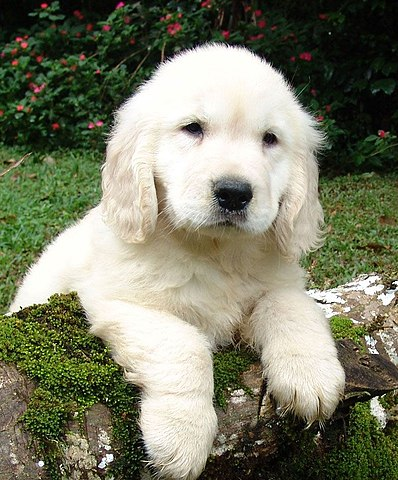
\includegraphics[width=20mm]{./figures/golden-retriever-puppy.jpeg}
      \caption{\centering Is this a [DOG]? \\ \tiny{Image from Wikipedia, \href{https://commons.wikimedia.org/w/index.php?curid=18521767}{Link}}}
    \end{figure}
    \vspace{-0.5cm}
    % \centering 
    \small{\emph{Prompt}: Is this a [DOG]?\\
    \emph{Expected Answer}: Yes}
  \end{columns}
\end{frame}
\note{
- Few-shot transfer is different from traditional machine learning that requires many examples \\
- The model doesn't actually learn in the traditional sense; it leverages knowledge from pre-training \\
- In this example, we show the model one example of a dog (a basset hound) and ask it to identify another dog \\
- This works because the model already knows what dogs look like from pre-training \\
- The quotation marks around 'learns' emphasize that it's not learning from scratch. I like to think of it as somehow narrowing the tree of possible responses from a point \\
}


% \subsection{Motivation}
\begin{frame}{Motivation}
\framesubtitle{Few-Shot Transfer}
  \vspace{-1em}
  \begin{columns}[T]
    \column{0.5\textwidth}
      \centering \emph{Fine-tuning}
      \begin{itemize}
        \item Requires significant computational resources, modifies model parameters
        \item Needs \emph{large(r) amounts} of \emph{labeled data}
        \item Can lead to catastrophic forgetting
        \item Refers to fine-tuning a pre-trained / instruction-tuned model on a specific task
      \end{itemize}
    \column{0.5\textwidth}
    \centering \emph{Few-shot Transfer}
    \begin{itemize}
        \item Uses \emph{`few' examples} or natural language \emph{descriptions}
        \item No model parameters are updated
        \item Potentially more practical for real-world applications~\footfullciteieee{Brown2020}
        \item Can be less effective for complex tasks
    \end{itemize}
  \end{columns}
\end{frame}
\note{
- Fine-tuning is the traditional approach for adapting pre-trained models to new tasks \\
- For VLMs, fine-tuning can require multiple high-end GPUs and days of compute time \\
- Catastrophic forgetting means the model may lose previously learned capabilities \\
- Few-shot transfer is much more efficient - we can use the model "as is" \\
- An important distinction: fine-tuning modifies the model weights, few-shot transfer doesn't \\
- The trade-off is that few-shot performance may not match fine-tuned performance for complex tasks \\
}


\subsection{Problem Statement}
\begin{frame}{Problem Statement}
\framesubtitle{Dataset Labeling for Computer Vision Tasks}
  \textbf{Challenge:} Creating labeled datasets to train specialized models for computer vision tasks is \emph{time-consuming} and \emph{expensive}~\footfullciteieee{Deng2009}, but VLMs are generalizable
  \vspace{0.5em}

  \textbf{Constraint:} However, VLMs are too \emph{computationally intensive} for direct deployment on resource-constrained environments (e.g., robots)
  \vspace{0.5em}
    
  \textbf{Opportunity:} VLMs could potentially automate label generation (\emph{pseudolabels}) to train \emph{downstream} models
  \vspace{1.2em}

  \centering \textbf{Research Question:} Can VLMs be transferred to generate \emph{pseudolabels} for computer vision tasks to train \emph{lightweight} downstream models?
  \blfootnote{\vspace{0.05em}}
\end{frame}
\note{
- The annotation of the ImageNet dataset required crowdsourcing to be feasible \\
- Specialized datasets like medical imaging can be even more expensive and require expert annotators \\
- VLMs require significant computational resources - multiple high-end GPUs with significant amounts of memory \\
- Most robots have limited computational capabilities - often a single low-power GPU or CPU \\
- Pseudolabels are automatically generated annotations that can be used in place of human-created labels \\
- The key insight: we don't need to deploy the large model - we use it to train a smaller, more efficient model \\
}
\section{Related Work}
\subsection{Background}
\begin{frame}{Related Work}
\framesubtitle{Development and Classes of Vision-Language Models}
  \vspace{-1em}
  \begin{columns}[T]
    \column{\customcolumnwidth}
    \textbf{VLM Classes}
    \vspace{-0.4em}
    \begin{itemize}
      \item \emph{Alignment models}: Generate unified text-image embeddings (CLIP~\footfullciteieee{Radford2021}, FLAVA) \vspace{-0.2em}
      \item \emph{Generative models}: Generate text conditioned on multimodal inputs (Flamingo, Frozen~\footfullciteieee{Tsimpoukelli2021}, MiniCPM~\footfullciteieee{Yao2024}, GPT-4o, Claude, etc.)
    \end{itemize}
    \column{\customcolumnwidth}
    \textbf{Architectural Approaches}
    \vspace{-0.4em}
    \begin{itemize}
      \item \emph{Towered}: Separate vision and language models with adapters
      \item \emph{Unified}: Single model processing both modalities "early on"~\footfullciteieee{ChameleonTeam2024}
    \end{itemize}
    \textbf{Key Insight}: Enables framing vision tasks as text generation~\footfullciteieee{Cho2021}, enabling streamlined task transfer
  \end{columns}
\end{frame}
\note{
- Vision-Language Models (VLMs) have progressed significantly since the introduction of CLIP \\
- Alignment models, such as CLIP, are designed to learn joint representations but do not generate textual outputs \\
- In contrast, generative models are capable of producing text responses based on visual inputs \\
- The Frozen model pioneered the approach of freezing the language model (LLM) while solely training the vision encoder \\
- Contemporary VLMs often incorporate separate pre-trained components for vision and language, connected through adapters or connectors \\
- Additionally, unified architectures that process both modalities simultaneously have emerged, enhancing the integration of vision and language tasks \\
- A pivotal advancement facilitating few-shot transfer is the conceptualization of vision tasks as text generation tasks \\
- This paradigm allows us to articulate tasks using natural language, eliminating the need for specialized architectures \\
- The rapid evolution of this field has led to the emergence of models like GPT-4o, which can comprehend and reason about complex visual scenarios \\
}


\begin{frame}{Related Work}
\framesubtitle{Transfer Learning \& Adaptation Techniques}
  \vspace{-1em}
  \begin{columns}[T]
    \column{\customcolumnwidth}
      \textbf{Prompting Techniques}: Crafting prompts to improve task performance~\footfullciteieee{Liu2023}
      \begin{itemize}
        \item In-context learning: Providing examples in context~\footfullciteieee{Brown2020}
        \item Chain-of-thought prompting for complex reasoning~\footfullciteieee{Wei2022}
      \end{itemize}
    \column{\customcolumnwidth}
      \textbf{Parameter-Efficient Fine-Tuning}: Typically requires more examples than few-shot regime
      \begin{itemize}
        \item Prefix-tuning: Optimizing task-specific prompt vectors~\footfullciteieee{Li2021}
        \item Low-Rank Adaptation (LoRA)~\footfullciteieee{Hu2021}: decomposes weight updates into smaller trainable matrices
      \end{itemize}
  \end{columns}
\end{frame}
\note{
- Prompting techniques are crucial for adapting models to new tasks without retraining \\
- In-context learning allows models to learn from examples without parameter updates \\
- Chain-of-thought prompting helps models break down complex tasks into simpler steps \\
- Parameter-efficient fine-tuning methods like prefix-tuning are valuable for low-resource settings \\
- These techniques are less explored in VLMs compared to NLP models \\
- Our research contributes by evaluating these methods in the context of VLMs for dataset annotation \\
}


\begin{frame}{Related Work}
\framesubtitle{Applications and Datasets}
  \vspace{-1em}
  \begin{columns}[T]
    \column{\customcolumnwidth}
      \textbf{Applicability of VLMs}
      \vspace{-0.4em}
      \begin{itemize}
        \item Large-scale pre-training enables generalization to various tasks
        \item Traditional DNNs trained for specific tasks
      \end{itemize}
      \textbf{LLMs for Data Annotation}
      \vspace{-0.4em}
      \begin{itemize}
        \item LLMs used to generate multimodal instruction-following data~\footfullciteieee{Liu2023a}
        \item Seen to outperform crowd-workers in data annotation tasks~\footfullciteieee{Gilardi2023}
      \end{itemize}
    \column{\customcolumnwidth}
      \textbf{Key Datasets}:
      Various datasets exist for various vision tasks.
      \begin{itemize}
        \item ImageNet, CIFAR-10~\footfullciteieee{Krizhevsky2009}: Object recognition
        \item Microsoft COCO: Detection, segmentation, captioning
        \item Derm7Pt~\footfullciteieee{Kawahara2019}: Specialized dermatology dataset
        \item MVTec: Anomaly detection
      \end{itemize}
  \end{columns}
\end{frame}
\note{
- VLMs are used in a wide range of vision tasks, leveraging their ability to generalize from large-scale pre-training \\
- Traditional DNNs are typically trained on specific datasets for specific tasks, limiting their generalization \\
- LLMs have been used to generate multimodal instruction-following data to train VLMs, enhancing dataset creation \\
- LLMs have been seen to outperform human annotators, providing more consistent and scalable data annotation \\
- Key datasets like ImageNet and CIFAR-10 are benchmarks for evaluating model performance on object recognition \\
- Specialized datasets like Derm7Pt are crucial for testing models on domain-specific tasks \\
- Our research leverages these datasets to evaluate the effectiveness of VLMs in generating pseudolabels for downstream tasks \\
}


\subsection{Research Gaps and Limitations}
\begin{frame}{Research Gaps and Limitations}
\framesubtitle{What do we address, and what could hinder our work?}
  \vspace{-1.2em}
  \begin{columns}[T]
    \column{\customcolumnwidth}
      \textbf{Gaps Addressed in Our Work}
      \vspace{-0.4em}
      \begin{itemize}
        \item Few-shot transfer of VLMs (in-context learning) less explored than NLP counterparts~\footfullciteieee{Liu2023}
        \item Dataset annotation applications~\footfullciteieee{Tan2024}:
        \begin{itemize}
          \item Use of VLMs for dataset annotation less explored
          \item Analysis of downstream vision models from VLM-generated pseudolabels
        \end{itemize}
      \end{itemize}
    \column{\customcolumnwidth}
      \textbf{Known VLM Limitations}
      \vspace{-0.4em}
      \begin{itemize}
        \item Systematic shortcomings in visual reasoning, spatial relationships, and perspective~\footfullciteieee{Tong2024}
        \item Inherits LLM issues~\footfullciteieee{Li2023c} such as hallucinations, ungrounded reasoning, prior biases~\footfullciteieee{Chochlakis2024}, sensitivity to input ordering
      \end{itemize}
  \end{columns}
\end{frame}
\note{
- Few-shot transfer capabilities of VLMs are less studied compared to LLMs in NLP \\
- Most VLM research focuses on zero-shot or fine-tuning approaches \\
- Our work systematically evaluates VLMs for dataset annotation: \\
  - Comprehensive evaluation of different prompting strategies \\
  - Analysis of pseudolabel quality and consistency \\
  - Impact on downstream model performance \\
- We acknowledge important VLM limitations: \\
  - Difficulty with spatial relationships and perspective \\
  - Inherited issues from LLMs like hallucinations \\
  - Biases from pre-training data making model ignore visual context \\
- These limitations highlight areas needing further research \\
- Something to note: this is a large field of research, and most of the research was done in the last 4-5 years \\
}
\section{Proposed Approach}
\begin{frame}{Proposed Approach}
\framesubtitle{Evaluating VLMs for Pseudolabel Generation}
  \textbf{Approach:} Evaluate VLMs on generating \emph{accurate pseudolabels} for image classification datasets under various \emph{zero-shot} and \emph{few-shot} transfer conditions
  \vspace{0.3em}
    
  \begin{columns}[T]
    \column{0.55\textwidth}
      \centering \textbf{Key Research Aspects}
      \begin{enumerate}
        \item How does the \emph{number of examples} (few-shot vs. zero-shot) affect pseudolabel quality?
        \item What are the \emph{computational requirements} for practical application?
        \item How effective are the \emph{downstream models} trained on pseudolabels?
      \end{enumerate}

    \column{0.45\textwidth}
    \begin{figure}
      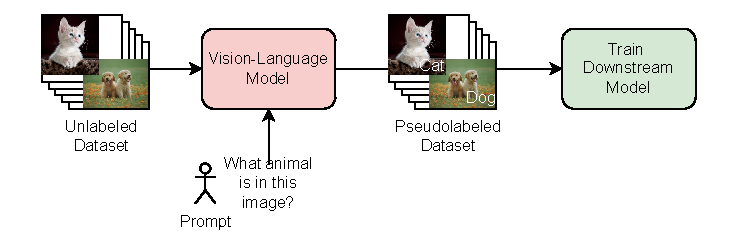
\includegraphics[width=\textwidth]{figures/vlm_transfer_downstream.pdf}
      \caption{\centering Using VLMs to generate pseudolabels for downstream model training}
    \end{figure}
  \end{columns}
\end{frame}
\note{
- Zero-shot means only describing the task in natural language; few-shot means providing examples \\
- We tested multiple prompting strategies to find the most effective approach \\
- We examined both common visual tasks (CIFAR-10) and specialized tasks (dermatology) to see if few-shot transfer is generalizable \\
- This design helps us understand when VLMs can be reliably transferred for automatic labeling \\
- For computational requirements, we measured inference time, memory usage, and scaling properties \\
- Downstream models were evaluated against models trained on ground truth labels \\
}


\section{Methodology}
\newcommand{\CifarDatasetSlide}{
\begin{columns}[T]
  \column{\customcolumnwidth}
    \textbf{Dataset Characteristics}
    \begin{itemize}
      \item 60,000 RGB images (32x32 pixels)
      \item 10 \emph{balanced} categories
      \item Standard split:
      \begin{itemize}
        \item 50,000 training
        \item 10,000 test (1,000/class)
      \end{itemize}
      % \item Categories:
      % \begin{itemize}
      %   \item Natural: birds, cats, deer, dogs, frogs, horses
      %   \item Artificial: airplanes, automobiles, ships, trucks
      % \end{itemize}
      \item \emph{Common} vision task
    \end{itemize}
  \column{\customcolumnwidth}
    \begin{figure}
    % CIFAR-10 examples figure
\begin{figure}[h]
  \begin{tabular}{ccccc}
    \begin{minipage}[b]{0.15\linewidth}
      
\includegraphics[width=\linewidth]{figures/cifar-images/airplane.png}
      \centering\scriptsize\texttt{airplane}
    \end{minipage} &
    \begin{minipage}[b]{0.15\linewidth}
      
\includegraphics[width=\linewidth]{figures/cifar-images/automobile.png}
      \centering\scriptsize\texttt{auto}
    \end{minipage} &
    \begin{minipage}[b]{0.15\linewidth}
      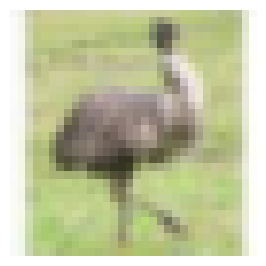
\includegraphics[width=\linewidth]{figures/cifar-images/bird.png}
      \centering\scriptsize\texttt{bird}
    \end{minipage} &
    \begin{minipage}[b]{0.15\linewidth}
      
\includegraphics[width=\linewidth]{figures/cifar-images/cat.png}
      \centering\scriptsize\texttt{cat}
    \end{minipage} &
    \begin{minipage}[b]{0.15\linewidth}
      
\includegraphics[width=\linewidth]{figures/cifar-images/deer.png}
      \centering\scriptsize\texttt{deer}
    \end{minipage} \\
    \begin{minipage}[b]{0.15\linewidth}
      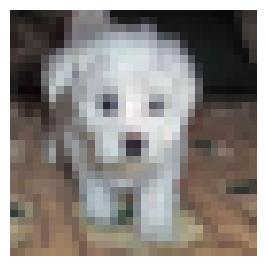
\includegraphics[width=\linewidth]{figures/cifar-images/dog.png}
      \centering\scriptsize\texttt{dog}
    \end{minipage} &
    \begin{minipage}[b]{0.15\linewidth}
      
\includegraphics[width=\linewidth]{figures/cifar-images/frog.png}
      \centering\scriptsize\texttt{frog}
    \end{minipage} &
    \begin{minipage}[b]{0.15\linewidth}
      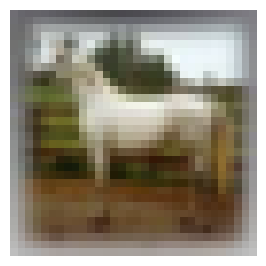
\includegraphics[width=\linewidth]{figures/cifar-images/horse.png}
      \centering\scriptsize\texttt{horse}
    \end{minipage} &
    \begin{minipage}[b]{0.15\linewidth}
      
\includegraphics[width=\linewidth]{figures/cifar-images/ship.png}
      \centering\scriptsize\texttt{ship}
    \end{minipage} &
    \begin{minipage}[b]{0.15\linewidth}
      
\includegraphics[width=\linewidth]{figures/cifar-images/truck.png}
      \centering\scriptsize\texttt{truck}
    \end{minipage}
  \end{tabular} 
\end{figure}
    \caption{Example images from CIFAR-10~\footfullciteieee{Krizhevsky2009}}
    \end{figure}
\end{columns}
}
\subsection{Datasets}
\begin{frame}{Datasets Used}
  \framesubtitle{CIFAR-10 Dataset}
  \vspace{-1em}
  \CifarDatasetSlide
\end{frame}
\note{

}

\newcommand{\DermPtDatasetSlide}[1]{
\begin{columns}[T]
  \column{\customcolumnwidth}
    \textbf{Dataset Characteristics}
    \vspace{-0.4em}
    \begin{itemize}
      \item 1,011 dermatological cases for melanoma diagnosis (as well as other skin conditions)
      \item Multiple image modalities:
        \begin{itemize}
          \item Dermoscopic (standardized)
          \item Clinical (varying conditions)
        \end{itemize}
      % \item Dataset split (diagnoses and features not uniform):
      %   \begin{itemize}
      %     \item 413 training cases
      %     \item 203 validation cases
      %     \item 395 test cases
      %   \end{itemize}
      \item Diagnoses and features are not uniformly distributed
      \item Task-specific dataset -- likely not present in VLM pre-training data
    \end{itemize}
  \column{\customcolumnwidth}
    \vspace{-0.5em}
    #1
\end{columns}
}

\newcommand{\DermPtFigureOne}{
  \begin{figure}[h]
    \centering
    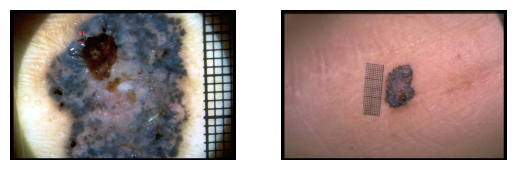
\includegraphics[width=0.9\linewidth]{figures/derm7pt-images/derm_01.png}
    \vspace{0.25em}
    \raggedright
    \scriptsize\texttt{diagnosis}: basal cell carcinoma\\
    \scriptsize\texttt{pigment\_network}: absent\\
    \scriptsize\texttt{streaks}: absent\\
    \scriptsize\texttt{pigmentation}: absent\\
    \scriptsize\texttt{regression\_structures}: blue areas\\
    \scriptsize\texttt{dots\_and\_globules}: irregular\\
    \scriptsize\texttt{blue\_whitish\_veil}: present\\
    \scriptsize\texttt{vascular\_structures}: within regression\\
    \vspace{0.25em}
    \scriptsize\texttt{seven\_point\_score}: 4\\
    \scriptsize\texttt{level\_of\_diagnostic\_difficulty}: low
    \caption{\centering An example case from Derm7Pt}
  \end{figure}
}

\newcommand{\DermPtFigureTwo}{
  \begin{figure}[h]
    \centering
    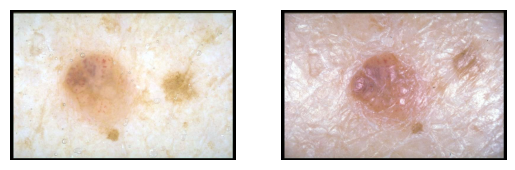
\includegraphics[width=0.9\linewidth]{figures/derm7pt-images/derm_02.png}
    \vspace{0.25em}
    \raggedright
    \scriptsize\texttt{diagnosis}: melanoma metastasis\\
    \scriptsize\texttt{pigment\_network}: absent\\
    \scriptsize\texttt{streaks}: absent\\
    \scriptsize\texttt{pigmentation}: diffuse irregular\\
    \scriptsize\texttt{regression\_structures}: absent\\
    \scriptsize\texttt{dots\_and\_globules}: regular\\
    \scriptsize\texttt{blue\_whitish\_veil}: absent\\
    \scriptsize\texttt{vascular\_structures}: hairpin\\
    \vspace{0.25em}
    \scriptsize\texttt{seven\_point\_score}: 1\\
    \scriptsize\texttt{level\_of\_diagnostic\_difficulty}: high
    \caption{\centering A particularly challenging example case from Derm7Pt}
  \end{figure}
}

\begin{frame}{Datasets Used}
  \framesubtitle{Seven-Point Checklist Dermatology Dataset (Derm7Pt)}
  \vspace{-1em}
  \DermPtDatasetSlide{\DermPtFigureOne}
\end{frame}
\note{
- The Derm7Pt dataset is a collection of dermatological images and annotations for melanoma diagnosis, as well as other skin conditions such as seborrheic keratosis, basal cell carcinoma, types of nevi, and more \\
- A seven point score of greater than or equal to 3 is to be referred for specialist analysis for melanoma \\
- The authors provide a python library as an interface to the dataset, and perform grouping of rare cases as well as the grouping of fine-grained categorization into more coarse categories \\
- In the authors' paper, it is shown that incorporating clinical images as input to their CNN model improves performance \\
}


\subsection{Models Chosen}
\begin{frame}{Models Chosen}
\framesubtitle{Which models did we evaluate?}
  \vspace{-1em}
  \begin{columns}[T]
    \column{\customcolumnwidth}
    \begin{itemize}
      \item \textbf{InternVL2-8B:} 8B parameters, 8k context window
      \item \textbf{MiniCPM-V-2.6:} 8B parameters, \emph{image token compression} with \emph{perceiver-resampler} architecture
      \item \textbf{Pixtral 12B:} 12B parameters, 128K context window, \emph{handles images natively}
    \end{itemize}
    \column{\customcolumnwidth}
    \begin{itemize}
      \item \textbf{Phi-3.5-Vision-Instruct:} 4B parameters, 128K context window, designed for constrained environments
      \item \textbf{Bio-Medical-MultiModal-Llama-3-8B-V1:} 8B parameters, \emph{fine-tuned} multimodal adaptation of Llama-3.1-8B-Instruct for \emph{biomedical} tasks
    \end{itemize}
  \end{columns}
  \textbf{Notes:}
  \begin{itemize}
    \setlength{\itemsep}{0em}
    \item All models use towered architectures, integrating visual encoders with language models, with \emph{integrated image} tiling, \emph{processing} methods (except for Pixtral)
    \item Models chosen for claimed ability in processing \emph{interleaved} image-text inputs
  \end{itemize}
\end{frame}
\note{
- InternVL2-8B and MiniCPM-V-2.6 models integrate visual and language processing components \\
- Phi-3.5-vision-instruct and Pixtral 12B models are designed for long-context multimodal processing \\
- Bio-Medical-MultiModal-Llama-3-8B-V1 is specialized for biomedical tasks \\
- Models selected for their ability to handle multi-image, multi-turn multimodal conversations, or in other words, interleaved text and image inputs \\
- Notably, all models use their own integrated image tiling and processing methods, except for the Pixtral 12B model, which processes images natively at their full resolution without tiling
}


\subsection{Experimental Design}
\begin{frame}{Experimental Design}
\framesubtitle{How did we evaluate VLMs?}
  \vspace{-1em}
  \begin{itemize}
    \item \textbf{Zero-Shot Transfer:}
    \begin{itemize}
      \item Evaluated ability to perform tasks \emph{without prior examples}
      \item Used basic and enhanced prompts with task-specific information and chain-of-thought reasoning
    \end{itemize}
    \item \textbf{Few-Shot Transfer:}
    \begin{itemize}
      \item Assessed effects of \emph{providing examples} on model performance, resource usage
      \item Explored pure few-shot experiments and combinations with prompting
    \end{itemize}
    \item \textbf{Downstream Model Training:}
    \begin{itemize}
      \item Evaluated \emph{knowledge transfer} by training downstream models from pseudolabels
      \item Analyzed effects of transfer methods on downstream model performance
    \end{itemize}
  \end{itemize}
\end{frame}
\note{
- Zero-shot learning assessed through basic and enhanced prompts \\
- Few-shot learning explored with varying examples and combinations \\
- Downstream training focused on pseudolabel effectiveness \\
- Comprehensive evaluation framework used to assess VLM capabilities \\
}


% \subsection{Prompting and VLM Inputs}
\begin{frame}{Prompting and VLM Inputs}
\framesubtitle{How did we prompt the VLM?}
  \vspace{-1em}
  A \emph{Prompting Framework} was developed, that:
  \begin{itemize}
    \item Employed a consistent \emph{chat-based} interaction format for fair comparison
    \item Isolated effects of different prompting components (zero-shot, few-shot, reasoning) with a \emph{modular} prompt structure
    \item \emph{Minimized biases} through systematic, deterministic and reproducible \emph{randomization} of class lists and example ordering
  \end{itemize}
\end{frame}
\note{
- Prompting strategy focused on fair comparison and isolating effects of different components \\
- Chat-based format maintained consistency across experiments \\
- Standardized preprocessing and prompt templates ensured reproducibility \\
- Deterministic random seeds used for example selection and class list shuffling \\
- Core structure included base prompt, example integration, and test instance presentation \\
}


\begin{frame}{Prompting and VLM Inputs}
\framesubtitle{How did we prompt the VLM?}
  \vspace{-1em}
  \begin{columns}[T]
    \column{\customcolumnwidth}
    \textbf{Core Structure of the Prompt:}
    \begin{itemize}
      \item \textbf{Base Prompt Structure:} \emph{Guides models} with task definition and output format
      \item \textbf{Example Integration:} Alternating user-assistant message pairs for \emph{few-shot examples}
      \item \textbf{Test Instance Presentation:} Test image presented for classification in \emph{final turn}
    \end{itemize}
    \column{\customcolumnwidth}
    \vspace{-4em}
    \begin{figure}
      \centering
      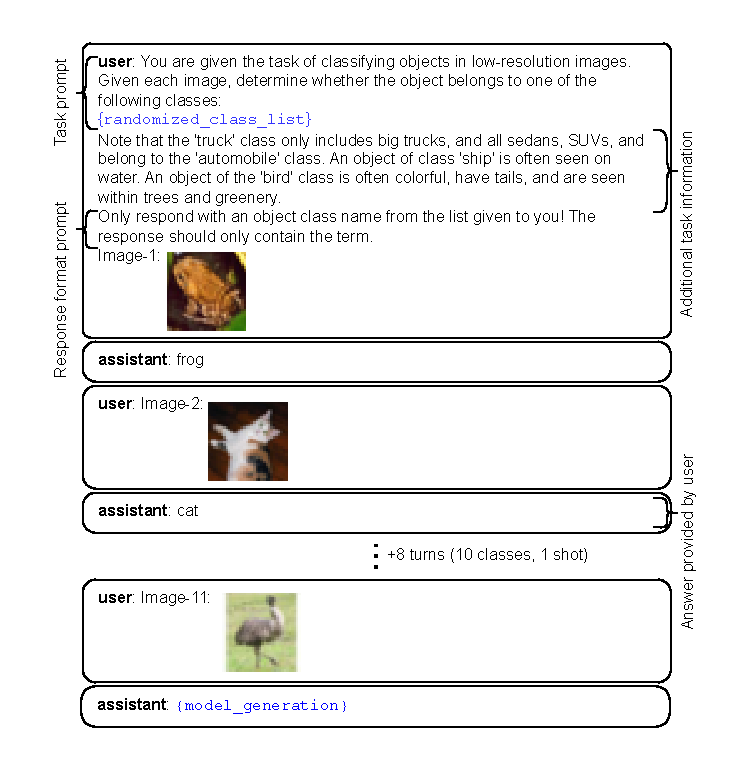
\includegraphics[width=1.12\linewidth]{figures/prompt_building.pdf}
      \vspace{-2.4em}
      \caption{Visualization of the prompt building process}
    \end{figure}
  \end{columns}
\end{frame}
\note{
- The example shown is for the CIFAR-10 dataset. A similar process is used for the Derm7Pt dataset, but with category-specific prompts for each category and the optional addition of clinical images \\
- Base prompt structure guides models with task definition, class list, reasoning requirements, and output format
- Alternating user-assistant message pairs for few-shot examples -- answers are provided by user
- Final turn presents test image for classification -- answer is provided by model
}
\section{Evaluation}
\subsection{CIFAR-10 Experiments}
\begin{frame}{CIFAR-10 Experiments}
\framesubtitle{A General Image Classification Task}
  \vspace{-1em}
  \CifarDatasetSlide
\end{frame}


\subsection{CIFAR-10 Experiments}
\begin{frame}{CIFAR-10 Experiments}
\framesubtitle{A General Image Classification Task}
  \vspace{-1em}
  \begin{columns}[T]
    \column{\customcolumnwidth}
      \textbf{Experimental Setup}
      \begin{itemize}
        \item Four VLMs evaluated:
        \begin{itemize}
          \item Pixtral 12B
          \item InternVL2
          \item MiniCPM v2.6
          \item Phi-3.5 Vision Instruct
        \end{itemize}
        \item Prompting strategies:
        \begin{itemize}
          \item Zero-shot with / without additional task information and chain-of-thought reasoning
          \item Few-shot (1-16 examples, with and without textual prompts)
        \end{itemize}
      \end{itemize}
    \column{\customcolumnwidth}
      \textbf{Key Findings}
      \begin{itemize}
        \item Zero-shot performance:
        \begin{itemize}
          \item Consistent across prompting strategies
          \item Reasoning requirements decreased accuracy by 10-15\%
        \end{itemize}
        \item Few-shot insights:
        \begin{itemize}
          \item Performance peaks at 4-8 examples
          \item Super-linear increase in resource usage
          \item Prompting improves low-shot scenarios
        \end{itemize}
      \end{itemize}
  \end{columns}
\end{frame}
\note{
- Evaluated four state-of-the-art VLMs on CIFAR-10 image classification \\
- Zero-shot experiments showed consistent performance across different prompting strategies \\
- Adding reasoning requirements actually decreased performance by 10-15\% due to format constraints and the limitations of some VLMs in following instructions \\
- Few-shot performance varied by model: Pixtral and InternVL2 showed improvements up to 8 examples \\
- MiniCPM and Phi-3.5 peaked earlier at 4-6 examples \\
- Resource usage increased super-linearly with number of examples \\
- Memory usage patterns varied: Pixtral showed super-linear increase, MiniCPM remained constant \\
- Processing time increased dramatically: 2 examples ~10x, 4 examples ~20x, 8 examples 30-50x longer than zero-shot \\
- Downstream models trained on pseudolabels often outperformed the VLMs themselves \\
}

\subsection{Downstream Model Analysis}
\begin{frame}{Downstream Model Analysis}
\framesubtitle{Performance Characteristics and Insights}
  \vspace{-1em}
  \begin{columns}[T]
    \column{\customcolumnwidth}
      \textbf{Performance Characteristics}
      \begin{itemize}
        \item Downstream models outperformed VLMs, possibly due to:
        \begin{itemize}
          \item Pre-trained ResNet-18 model~\footfullciteieee{He2016}
          \item Focus on pattern recognition compared to image-text modeling
        \end{itemize}
        % Rework this section, it is not clear at all
        \item Label quality vs. dataset size:
        \begin{itemize}
          \item Quality more crucial than quantity
          \item 90\% VLM accuracy threshold
        \end{itemize}
      \end{itemize}
    \column{\customcolumnwidth}
      \textbf{Key Insights}
      \begin{itemize}
        \item Weak dependence of performance on shot count
        \item Embracing noise: label smoothing improved performance by \(\sim\)1\%
        \item Practical implications:
        \begin{itemize}
          \item Zero/low-shot approaches sufficient
          \item Simple prompts more effective
          \item High resilience to label noise
        \end{itemize}
      \end{itemize}
  \end{columns}
\end{frame}
\note{
- Downstream models consistently outperformed VLMs due to ImageNet pre-training and focus on pattern recognition \\
- Performance showed weak dependence on number of examples used in VLM predictions \\
- Models maintained good performance even with lower-quality labels from 1-shot experiments \\
- Label quality proved more important than dataset size in training \\
- Models trained on limited but accurate ground truth labels performed better until VLM accuracy reached ~90\% \\
- Practical finding: zero-shot or low-shot (1-2 examples) with prompting is most efficient implementation strategy \\
- Higher shot counts showed diminishing returns despite increased computational costs \\
- Downstream models showed remarkable resilience to label quality, suggesting practical utility even with imperfect data \\
}


\subsection{Seven-Point Checklist Dermatology Experiments}
\begin{frame}{Dermatology Experiments}
\framesubtitle{Experiment Setup and Evaluation Framework}
  \vspace{-1em}
  \DermPtDatasetSlide{\DermPtFigureOne}
\end{frame}


\begin{frame}{Dermatology Experiments}
\framesubtitle{Experiment Setup and Evaluation Framework}
  \vspace{-1em}
  \begin{columns}[T]
    \column{\customcolumnwidth}
      \textbf{Experimental Setup}
      \begin{itemize}
        \item Five VLMs evaluated:
        \begin{itemize}
          \item Pixtral 12B, InternVL2
          \item MiniCPM v2.6, Phi-3.5
          \item Biomedical Multimodal Model (domain-specific, fine-tuned model)
        \end{itemize}
        \item Two experiment types:
        \begin{itemize}
          \item Direct diagnosis of condition
          \item Structured feature understanding (7-point checklist with category-specific prompts)
        \end{itemize}
      \end{itemize}
    \column{\customcolumnwidth}
      \textbf{Evaluation Framework}
      \begin{itemize}
        \item Multiple image modalities:
        \begin{itemize}
          \item Dermoscopic images (standardized)
          \item Clinical images (varying conditions, optional)
        \end{itemize}
        \item Prompting strategies:
        \begin{itemize}
          \item Zero-shot with/without reasoning
          \item Few-shot (1-8 examples with and without textual prompts)
          \item Optional: additional task information in structured prompting (0.5-shot)
        \end{itemize}
      \end{itemize}
    \end{columns}
\end{frame}

\begin{frame}{Dermatology Experiments}
\framesubtitle{Key Findings}
  \vspace{-1em}
  \begin{columns}[T]
    \column{\customcolumnwidth}
      \textbf{Performance Patterns}
      \begin{itemize}
        \item Most models near random-guess accuracy
        \item Domain-specific model struggled significantly, with poor instruction following
        \item Clinical images often degraded performance
      \end{itemize}
    \column{\customcolumnwidth}
      \textbf{Key Challenges}
      \begin{itemize}
        \item Limited pre-training knowledge
        \item Multi-modal integration issues
        \item Performance degradation with:
        \begin{itemize}
          \item Increased examples
          \item Added reasoning requirements
          \item Multiple image modalities (addition of clinical images)
        \end{itemize}
      \end{itemize}
  \end{columns}
\end{frame}
\note{
- Most models near random-guess accuracy, indicating fundamental limitations of VLMs for this task \\
- The domain-specific Biomedical Multimodal Model struggled, and this is likely because the fine-tuning caused regressions in the instruction-following capabilities of the model. This is somewhat of a known issue, and goes along the lines of catastrophic forgetting -- but this is something that a few-shot or zero-shot transferred model may not suffer from \\
- It seems we are at the limits of what and how much can be provided as inputs to the model, as well as the knowledge of the model itself \\
}

\begin{frame}{Dermatology Experiments}
\framesubtitle{Structured vs Direct Diagnosis}
  \begin{columns}[T]
    \column{\customcolumnwidth}
      \textbf{Direct Diagnosis Approach}
      \begin{itemize}
        \item Zero-shot baseline:
          \begin{itemize}
            \item Only Pixtral 12B above random
            \item Reasoning decreased performance
          \end{itemize}
        \item Few-shot performance:
          \begin{itemize}
            \item Some improvement over zero-shot
            \item Diminishing returns with examples
          \end{itemize}
      \end{itemize}
    \column{\customcolumnwidth}
    % This is incomplete, refine this, add zero-shot performance
      \textbf{Structured Prompting} on seven-point checklist categories
      \begin{itemize}
        \item Few-shot performance:
          \begin{itemize}
            \item Generally inferior to zero-shot
            \item Peak at 2-4 examples for most models
            % Verify this
            % \item Limited benefit from task-specific info
          \end{itemize}
      \end{itemize}
  \end{columns}
\end{frame}
\note{
- The Derm7Pt experiments revealed significant challenges in applying VLMs to specialized medical tasks \\
- Most models performed at or around random-guessing accuracy, indicating fundamental limitations \\
- Adding clinical images alongside dermoscopic images often degraded performance \\
- Even the domain-specific Biomedical Multimodal Model struggled significantly \\
- Resource requirements increased substantially with experiment complexity \\
- Direct diagnosis showed some promise with few-shot learning, while structured prompting was generally less effective \\
- These findings suggest current VLMs need significant improvements for specialized medical tasks \\
- The results highlight the importance of pre-existing task knowledge in few-shot learning success \\
}

\begin{frame}{Implications and Conclusions}
\framesubtitle{What did we learn from the experiments?}
  \vspace{-1em}
  \begin{columns}[T]
    \column{\customcolumnwidth}
      \textbf{Key Insights}
      \begin{itemize}
        \item Pre-training knowledge crucial:
          \begin{itemize}
            \item Poor performance on specialized tasks
            \item Transferability to specialized domains not guaranteed
          \end{itemize}
        \item Architectural considerations:
          \begin{itemize}
            \item Model size \(\nRightarrow\) performance
            \item Multi-modal integration challenges exist
          \end{itemize}
        \item Few-shot transfer is closer to task \emph{recognition} than task learning
      \end{itemize}
    \column{\customcolumnwidth}
      \textbf{Future Directions} -- specialized training needed:
      \begin{itemize}
        \item for domain-specific pre-training
        \item to improve multi-modal integration
      \end{itemize}
      \textbf{Practical Considerations}
      \begin{itemize}
        \item Prefer simpler prompting strategies
        \item Consider resource-performance trade-offs
        \item Formulate task-specific evaluation metrics
        \item Models pre-trained on multi-image, multi-turn conversation -- better
      \end{itemize}
  \end{columns}
\end{frame}
\note{
- Context length and memory limitations restricted few-shot experiments to limited examples and constrained larger models \\
- Observed trends already show limited/degraded performance scaling with higher number of examples \\
- Poor performance on specialized domains suggests models rely more on pre-trained priors than learning new capabilities \\
- Promising research directions include investigating domain-specific pre-training strategies \\
- Each kind of image is a different modality in the dermatology case. The model may not know how to look at both image which are two forms of the same thing, and reason and understand the relationship between the two. The integration of the two modalities is a challenge. How do you look at to forms of the same thing and reason about the relationship between the two? \\
}

\subsection{Compute Analysis}
\begin{frame}{Compute Analysis}
\framesubtitle{Analysis of Memory and Processing Time}
  \vspace{-1em}
  \begin{columns}[T]
    \column{\customcolumnwidth}
      \textbf{Memory Usage Patterns}
      \begin{itemize}
        \item Model-dependent scaling:
        \begin{itemize}
          \item Pixtral 12B: \emph{Super-linear} increase
          \item InternVL2, Phi-3.5: \emph{Linear} scaling
          \item MiniCPM: \emph{Near-constant} (perceiver-resampler)
        \end{itemize}
        \item Clinical images (dermatology experiments): 1-1.75x increase
        \item \emph{Less} than the expected \emph{quadratic} scaling for pure transformers~\footfullciteieee{Vaswani2017}
      \end{itemize}
    \column{\customcolumnwidth}
      \textbf{Processing Time Impact}
      \begin{itemize}
        \item Near-linear increase with examples (compared to zero-shot):
        \begin{itemize}
          \item 2 examples: \(\sim\)10x longer
          \item 4 examples: \(\sim\)20x longer
          \item 8 examples: 30-50x longer
        \end{itemize}
        \item Reasoning requirements: 10-35\% longer
        \item Clinical images (dermatology experiments): 1.5-2.5x longer
      \end{itemize}
  \end{columns}
\end{frame}
\note{
- Memory usage patterns vary significantly between model architectures \\
- Pixtral 12B shows super-linear memory scaling with number of examples, likely due to pure transformer architecture \\
- InternVL2 and Phi-3.5 show more manageable linear scaling patterns \\
- MiniCPM's perceiver-resampler architecture enables near-constant memory usage regardless of examples \\
- Clinical images (additional images) increase memory usage by 1-1.75x \\
- Processing time increases dramatically with number of examples used \\
- Adding reasoning requirements (e.g., chain-of-thought) increases processing time by 10-35\% due to the generation of more output tokens \\
- Clinical images take 1.5-2.5x longer to process due to increased number of images and complexity \\
- These patterns align with theoretical expectations for optimized transformer architectures, and are lower than the expected quadratic scaling \\
}


\begin{frame}{Compute Analysis}
\framesubtitle{Practical Implications}
  \vspace{-1em}
  \begin{columns}[T]
    \column{\customcolumnwidth}
      \textbf{Resource-Performance Trade-offs} -- Diminishing returns with examples:
      \begin{itemize}
        \item Performance peaks at 4-8 examples
        \item Resource costs can grow super-linearly
      \end{itemize}
    \column{\customcolumnwidth}
      \textbf{Recommendations} -- Optimizing for practical deployment:
      \begin{itemize}
        \item Zero-shot or 1-2 shots with prompting
        \item Avoid reasoning requirements (unless the task calls for it)
        \item Single-image-per-turn processing when possible
      \end{itemize}
  \end{columns}
  \vspace{1em}
  \textbf{Architecture and model pre-training considerations:}
    \begin{itemize}
      \item Perceiver-resampler based models more efficient
      \item Larger model size \(\nRightarrow\) better performance
    \end{itemize}
\end{frame}
\note{
- Resource costs grow much faster than performance improvements with additional examples \\
- Perceiver-resampler architectures (like in MiniCPM) show better memory efficiency \\
- However, there may be a trade-off between resource efficiency and model performance \\
- Zero-shot or low-shot (1-2 examples) provides best balance of performance vs. resources \\
- Avoiding reasoning requirements saves significant processing time without major performance loss \\
- Why does reasoning not work? The tasks we chose are not reasoning-heavy tasks, but rather test visual recognition and grounding capabilities. Ungrounded reasoning cannot improve the recognition and grounding capabilties of the model \\
- Multi-image processing (e.g., clinical + dermoscopic) significantly impacts resources \\
- Architecture choice crucial for scaling to larger datasets or more complex tasks \\
- These findings help inform practical deployment strategies for VLMs in real applications \\
}
\section{Conclusions}
% \subsection{Key Findings}
\begin{frame}{Key Findings}
\framesubtitle{What did we learn about VLM few-shot transfer?}
  \vspace{-0.4em}
  \begin{columns}[T]
    \column{\customcolumnwidth}
      \textbf{General Domain (CIFAR-10)}
      \vspace{-0.2em}
      \begin{itemize}
        \item VLMs show \emph{fairly good transfer} to this task
        \item Downstream models achieve near ground-truth performance
        \begin{itemize}
          \item Only 5\% below models trained from ground-truth
          \item \emph{Resilient} to pseudolabel noise
          % \item Outperform VLMs in most cases
        \end{itemize}
      \end{itemize}
    \column{\customcolumnwidth}
      \textbf{Specialized Domain (Derm7Pt)}
      \vspace{-0.2em}
      \begin{itemize}
        \item \emph{Limited transfer} to specialized domains (Derm7Pt)
        \begin{itemize}
          \item Performance near random-guessing
          \item Suggests \emph{strong reliance} on pre-trained knowledge
        \end{itemize}
        \item Multi-modal \emph{integration challenges} exist
      \end{itemize}
  \end{columns}
  % \vspace{0.2em}
  \textbf{We find:}
  \begin{itemize}
    \item Zero / low-shot approaches with \emph{simple prompting} most effective
    \item Simpler prompting strategies generally outperform complex ones
    \item Examples help model \emph{recognize} the task (from pre-trained priors)~\footfullciteieee{Pan2023}
  \end{itemize}
  \vspace{-0.4em}
  \blfootnote{\vspace{0.05em}}
\end{frame}
\note{
- Zero-shot and low-shot approaches with simple prompting proved most effective for general domain tasks \\
- However, performance degraded significantly on specialized medical tasks (Derm7Pt). The domain is likely underrepresented in the pre-training data of the VLMs \\
- Architecture choices significantly impacted both performance and resource efficiency, e.g. the Perceiver-resampler architecture used in one of our models performs quite well, accuracy, memory, and time-wise \\
- Additional shots or reasoning requirements often increased costs without proportional gains \\
- Results suggest focusing on activating existing capabilities and knowledge rather than teaching new ones \\
- Each kind of image is a different modality in the dermatology case. The model may not know how to look at both image which are two forms of the same thing, and reason and understand the relationship between the two. The integration of the two modalities is a challenge. How do you look at to forms of the same thing and reason about the relationship between the two? \\
}


\begin{frame}{Key Contributions}
\framesubtitle{How did we help?}
  \vspace{-1em}
  \begin{itemize}
    \item Advancing the understanding of \emph{few-shot transfer} of VLMs:
    \begin{itemize}
      \item providing a comprehensive \emph{evaluation framework} for assessing VLM transfer
      \item providing \emph{practical guidelines} for their transfer to dataset annotation tasks to train task-specific downstream models
    \end{itemize}
    \item Empirical findings suggest downstream models are \emph{resilient to label noise}:
    \begin{itemize}
      \item significant for deploying these systems in \emph{resource-constrained} environments
      \item suggests that VLMs \emph{can} support the learning of smaller, task-specific models despite imperfect predictions
    \end{itemize}
  \end{itemize}
\end{frame}
\note{}


% \subsection{Limitations and Future Work}
\begin{frame}{Limitations and Future Work}
\framesubtitle{What constrained us, and what could be worked upon?}
  \vspace{-1em}
  \begin{columns}[T]
    \column{\customcolumnwidth}
      \textbf{Technical Limitations}
      \begin{itemize}
        \item Context length and memory constraints
        \item Limited / \emph{degraded performance scaling} with number of examples
        \item \emph{Limited generalization} to specialized domains
      \end{itemize}
      \textbf{General Limitations}
      \begin{itemize}
        \item Limited selection of models, datasets, tasks
        \item Findings of this work may not generalize to all vision tasks
      \end{itemize}
      \column{\customcolumnwidth}
      \textbf{Future Research Directions}
      \begin{itemize}
        \item Generalizable \emph{domain-transferable} pre-training strategies
        \item More \emph{efficient} VLM architectures for multi-image processing
        \item Improving prompting strategies and \emph{visual grounding}~\footfullciteieee{Yang2023}
        \item Extending investigation to \emph{other vision tasks}
      \end{itemize}
  \end{columns}
\end{frame}
\note{
- Context length and memory limitations restricted few-shot experiments to limited examples and constrained larger models, and high resolution images had to be rescaled to fit more examples \\
- Poor performance on specialized domains suggests models rely more on pre-trained priors than learning new capabilities \\
- There are some things that you can tell beforehand are bad ideas, and this was not specifically one of them. We expected before starting the project that more examples would strictly improve performance, but this was not the case. In NLP and LLMs, few-shot transfer and chain-of-thought prompting is extremely effective, but this is not the case for vision-language models and vision-language tasks, as we see here. \\
- More efficient VLM architectures needed for scalable high-resolution multi-image processing. Not only this, but for the use of VLMs and VLAs in robots in general, the ability to process multiple images at once and keep them in context is extremely important. \\
- Other vision tasks to try: object detection, segmentation, captioning to support a contrastive learner, etc.
}


% \section{Q\&A}
\begin{frame}{Thank You!}
  \vspace{6em}
  \centering
  \vfill
  {\LARGE \textbf{Questions?}}
  \vfill
  \vspace{6em}
  \raggedright\textbf{Contact:}
  \begin{itemize}
    \item shinas.shaji@smail.inf.h-brs.de
    \item shinas.shaji@iais.fraunhofer.de
  \end{itemize}
  \vfill
\end{frame}
\note{
Q: Why were advanced models such as GPT-4o and other closed-source models not used in the work? \\
A: Multiple reasons: \\
- compute analysis cannot be performed, as memory usage cannot be read, times are dependent on network, and the size of the model is unknown \\
- we focus on open-source models, for whom the architectural details are known. This enables us to see, for example, that the perciever-resampler architecture used in one of our models performs quite well, accuracy, memory, and time-wise \\
- we cannot be sure that our datasets are in the dataset training mix for closed-source models. Open-source work typically also mentions the training data mix and datasets used. Remember, we needed to check how few-shot learning performs when we know that similar tasks are not in the pre-training data for the model \\
- closed-source models can get quite expensive when we need to push a whole dataset through them. We can however use batched inferences for half the cost. However, the code and processing would require overhauls to support this, and this was perhaps beyond scope
}

\end{document}
